\hypertarget{nb:moreva-vs-qm}{%
\section{Comparison with ordinary
QM, with phase correction and plotting}\label{nb:moreva-vs-qm}}

Conversions from symbolic to numeric (including implicit one) for
plotting seems problematic, either with \verb#subs()#
or \verb#lambdify()#, therefore we start over, with a
new notebook. We also assume \begin{equation*}
    \hbar = \omega = 1 \,\text{.}
\end{equation*}

\begin{lstlisting}[language=Python]
import numpy as np
from scipy.linalg import expm
\end{lstlisting}

\begin{lstlisting}[language=Python]
import matplotlib as mpl
from mpl_toolkits.mplot3d import Axes3D
import numpy as np
import matplotlib.pyplot as plt
\end{lstlisting}

\begin{lstlisting}[language=Python]
%matplotlib inline
\end{lstlisting}

\begin{lstlisting}[language=Python]
Hs = np.array([
    [0, 1j],
    [-1j, 0]
])
\end{lstlisting}

\begin{lstlisting}[language=Python]
def evolve_psi(t, t0, psi0):
    return expm(-1j*Hs*(t-t0)).dot(psi0)
\end{lstlisting}

\begin{lstlisting}[language=Python]
def correction_eigenJ(-t, t0, eigenvalue):
    return np.exp(1j*eigenvalue*(t-t0))
\end{lstlisting}

\begin{lstlisting}[language=Python]
def correction_timeshift(t, t0, timeshift):
    deltaT = np.pi/2
    omega_prime = (np.pi*timeshift) / (deltaT**2)
    return np.exp(-1j*omega_prime*(t-t0))
\end{lstlisting}

\begin{lstlisting}[language=Python]
def psi_fixed(t, t0, psi0, eigenvalue):
    return evolve_psi(t, t0, psi0) * correction_eigenJ(t, t0, eigenvalue) * correction_timeshift(t, t0, t0)
\end{lstlisting}

\begin{lstlisting}[language=Python]
def psi_fixed_0_re(t, t0, psi0, eigenvalue):
    return np.real(psi_fixed(t, t0, psi0, eigenvalue)[0])
\end{lstlisting}

\begin{lstlisting}[language=Python]
def psi_fixed_0_im(t, t0, psi0, eigenvalue):
    return np.imag(psi_fixed(t, t0, psi0, eigenvalue)[0])
\end{lstlisting}

\begin{lstlisting}[language=Python]
def psi_fixed_1_re(t, t0, psi0, eigenvalue):
    return np.real(psi_fixed(t, t0, psi0, eigenvalue)[1])
\end{lstlisting}

\begin{lstlisting}[language=Python]
def psi_fixed_1_im(t, t0, psi0, eigenvalue):
    return np.imag(psi_fixed(t, t0, psi0, eigenvalue)[1])
\end{lstlisting}

\begin{lstlisting}[language=Python]
mpl.rcParams['legend.fontsize'] = 10

fig = plt.figure(figsize=(15, 11))
ax = fig.gca(projection='3d')

# Prepare arrays x, y, z
# z is t
z = np.linspace(-np.pi/4, 3*np.pi/4, 500)

# Auto-broadcasting doesn't work as expected, therefore we explicitly
# map the z vector via `np.vectorize()`

# x is real part of psi[0] or Re(psi_H) as in psi = psi_H|H> + psi_V|V>
x = np.vectorize(lambda t: psi_fixed_0_re(t, -np.pi/4, [0, -1j], 0))(z) 
# y is imag part of psi[0] or Im(psi_H) as in psi = psi_H|H> + psi_V|V>
y = np.vectorize(lambda t: psi_fixed_0_im(t, -np.pi/4, [0, -1j], 0))(z) 

plt.plot([0, 0], [0, 0], [-np.pi/4, 3*np.pi/4], lw=1, c='pink', label='Time (clock cycle)')

ax.plot(x, y, z, label='\psi_H "rephased"')

points_x = np.array([     0.0,     1.0,       0.0])
points_y = np.array([     0.0,     0.0,       0.0])
points_z = np.array([-np.pi/4, np.pi/4, 3*np.pi/4])
ax.scatter(points_x, points_y, points_z, marker='^', c='red', s=50, alpha=1.0, label='discrete PW')

plt.xlabel(s='Re <H|psi>')
plt.ylabel(s='Im <H|psi>')
ax.set_zlabel('t')

ax.legend()

plt.show()
\end{lstlisting}

\begin{figure}
\centering
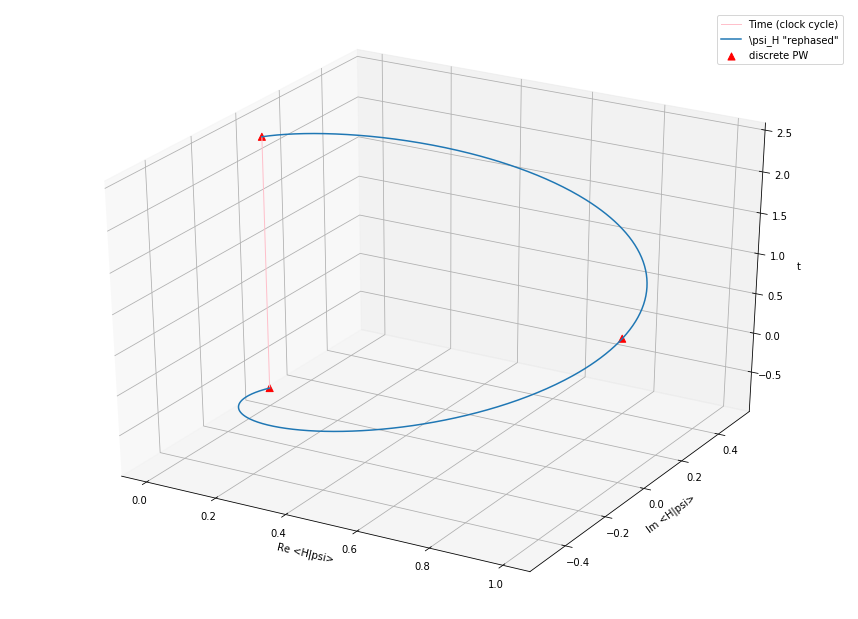
\includegraphics[width=\textwidth/2]{img/psi_H.png}
\caption[]{png}{png}
\end{figure}

\begin{lstlisting}[language=Python]
mpl.rcParams['legend.fontsize'] = 10

fig = plt.figure(figsize=(15, 11))
ax = fig.gca(projection='3d')

# Prepare arrays x, y, z
# z is t
z = np.linspace(-np.pi/4, 3*np.pi/4, 500)

# Auto-broadcasting doesn't work as expected, therefore we explicitly
# map the z vector via `np.vectorize()`

# x is real part of psi[1] or Re(psi_V) as in psi = psi_H|H> + psi_V|V>
x = np.vectorize(lambda t: psi_fixed_1_re(t, -np.pi/4, [0, -1j], 0))(z) 
# y is imag part of psi[0] or Im(psi_H) as in psi = psi_H|H> + ps_V|V>
y = np.vectorize(lambda t: psi_fixed_1_im(t, -np.pi/4, [0, -1j], 0))(z) 

plt.plot([0, 0], [0, 0], [-np.pi/4, 3*np.pi/4], lw=1, c='pink', label='Time (clock cycle)')

ax.plot(x, y, z, label='psi_V "rephased"')

points_x = np.array([     0.0,     0.0,       0.0])
points_y = np.array([    -1.0,     0.0,      -1.0])
points_z = np.array([-np.pi/4, np.pi/4, 3*np.pi/4])
ax.scatter(points_x, points_y, points_z, marker='^', c='red', s=50, alpha=1.0, label='discrete PW')

plt.xlabel(s='Re <V|psi>')
plt.ylabel(s='Im <V|psi>')
ax.set_zlabel('t')

ax.legend()

plt.show()
\end{lstlisting}

\begin{figure}
\centering
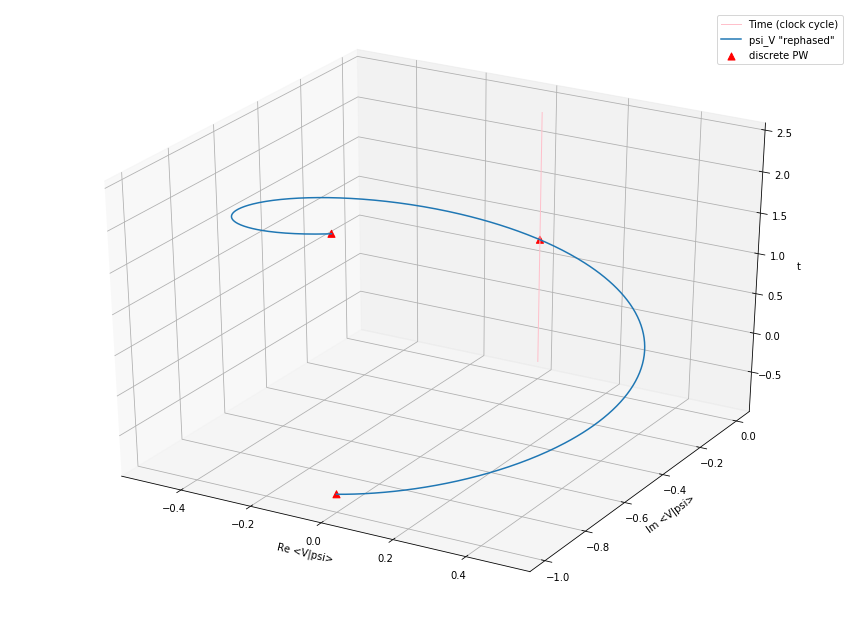
\includegraphics[width=\textwidth/2]{img/psi_V.png}
\caption[]{png}{png}
\end{figure}
